\vspace{-2.5cm}
\begin{tikzpicture}
    \node (physics) [blurb] {
    \vspace{5pt}
    \textcolor{black}{
    \newline{\fontsizetitle Physics of Advanced Reactors}\\
    \vspace{-20pt}\rule{\textwidth}{5pt}\\
    \fontsizesection
    Variance reduction methods for time-dependent Monte Carlo neutron transport. \\
        \vspace{20pt}
    Updated models of DNP group parameters for Molten Salt Reactors. \\
        \vspace{20pt}
    Computational modeling of flowing pebble-bed reactor systems.
        \begin{center}
        \begin{minipage}{.2\linewidth}
            
\includegraphics[height = 3\textwidth]{img/ghastly1.png}
        \end{minipage}
        \hspace{.5cm}
        \begin{minipage}{.2\linewidth}
            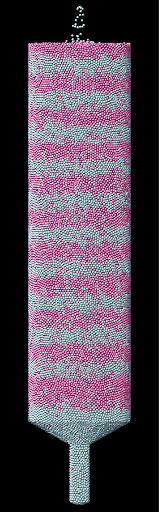
\includegraphics[height = 3\textwidth]{img/ghastly2.png}
        \end{minipage}
        \hspace{.5cm}
        \begin{minipage}{.2\linewidth}
            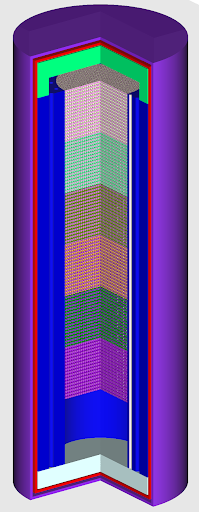
\includegraphics[height = 3\textwidth]{img/ghastly3.png}
        \end{minipage}
        \vspace{10pt}
        \figcaption{Simulation of a generic pebble bed HTGR core being filled (left) and online pebble recirculation (middle) using LAMMPS, 
        and a Xe-100-like full-core pebble bed HTGR (right) using SCALE \cite{richter}.}
        \end{center}
    }
    };
    \node (cycles) [blurb, below of = physics, yshift = -35.70cm] {
    \vspace{5pt}
    \textcolor{black}{
    \newline{\fontsizetitle Fuel Cycle and Energy System Optimization}\\
    \vspace{-20pt}\rule{\textwidth}{5pt}\\
    \fontsizesection
    Modeling and simulating scaled isotopic consequences of deploying Accelerators Driven Systems.\\
        \vspace{20pt}
    Techno-economic analysis of hybrid nuclear renewable energy systems (e.g. hydrogen microgrids).
        \begin{center}
        \begin{minipage}{.7\textwidth}
            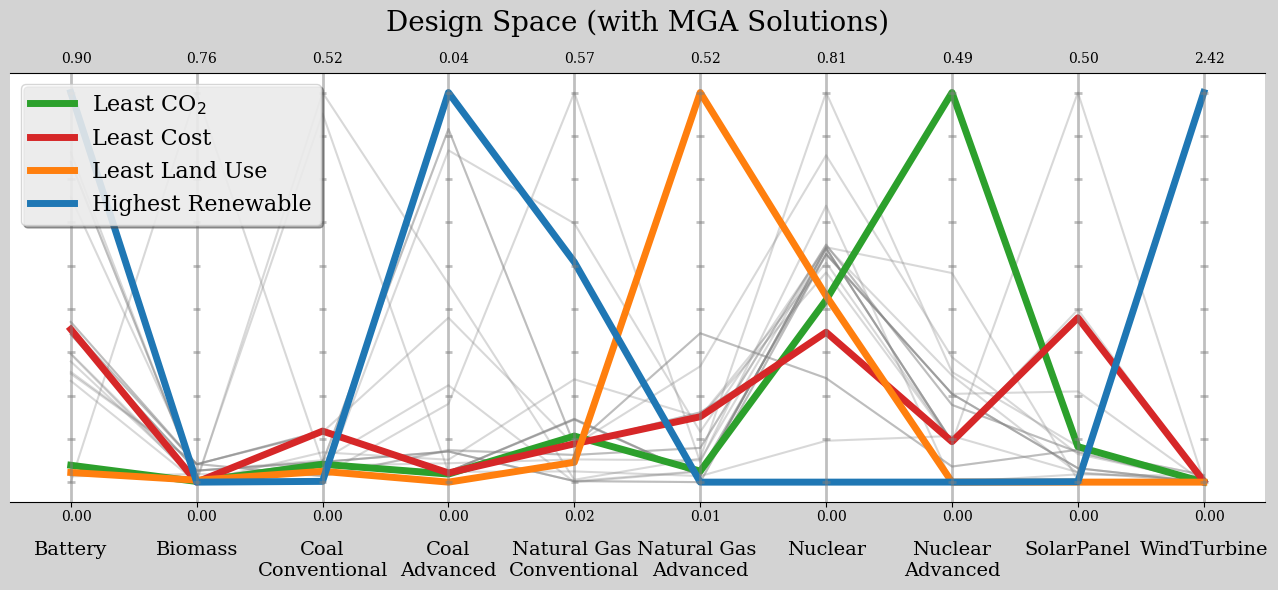
\includegraphics[width = \textwidth]{img/osier.png}
        \end{minipage}
        \vspace{10pt}
        \figcaption{The design space for a four objective problem including alternative solutions suggested by MGA.}
        \end{center}
        \vspace{20pt}
    Fuel cycle transition scenarios for advanced reactors.
        \begin{center}
        \begin{minipage}{.6\textwidth}
            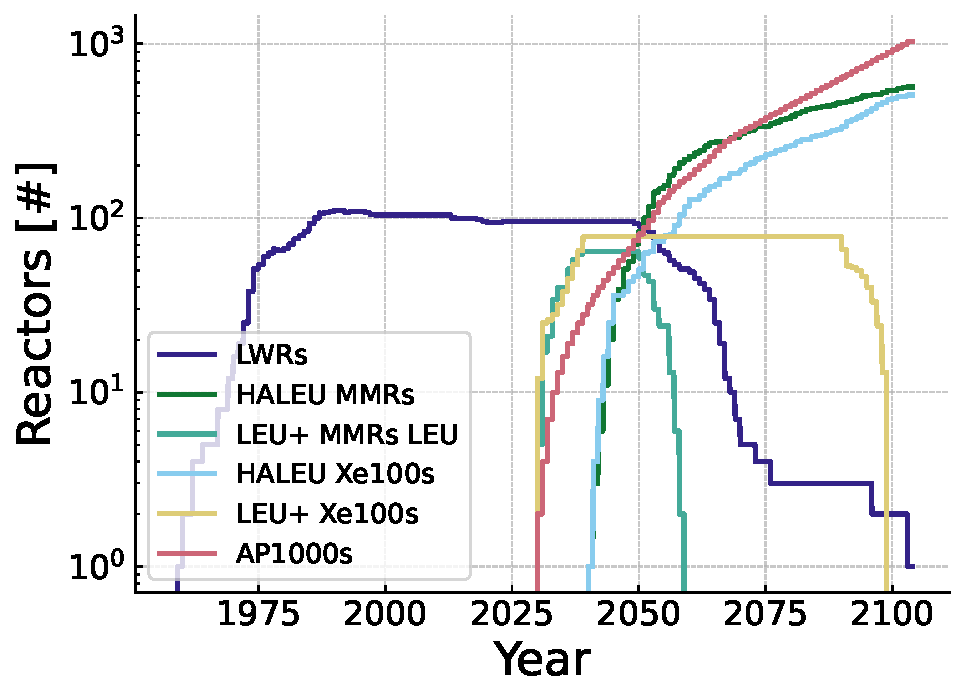
\includegraphics[width = \textwidth]{img/multi_dg2_reactors.pdf}
        \end{minipage}
        \vspace{10pt}
        \figcaption{Greedy AP1000 deployment along with Xe-100s and MMRs fueled by LEU+ and HALEU fuel.}
        \end{center}
    }
    };
\end{tikzpicture}